\chapter{Introduction}

For several years, in the field of Computational Biology, extensive research has been done on the efficient representation, indexing and annotation of linear genomes. Many researchers are now shifting towards graph-based representations since they give the additional benefit of representing collections and populations of genomes conveniently as well. However, there are many unsolved computational problems regarding this category of representation. I’ve worked on two particular problems. The first is succinct representation of membership information in a colored de Bruijn graph, and the second is efficient indexing for \kmers in a compacted de Bruijn graph. Below I provide a brief overview of research in the area and previous works on graph-based representation, along with common use cases of the various algorithms and methods developed.


\section{De Bruijn Graph}
\label{subsec:dbg}
Previous works have looked at how to represent populations and collections of genomes, along with variation detection in them~\cite{paten2017genome}. Graphs are nowadays very popular assets to represent sequences. They can be built on raw sequencing read data or reference genome strings. One can spell out different sequences by a walk through the nodes and edges of the graph, and this characteristic of a graph makes it a natural choice to represent collections of sequences. Furthermore, by putting together the paths extracted from a collection of sequences (e.g. sequencing reads) we can build up a giant graph which can be representative of the original reference for this pool of sequences (such as the underlying genome or transcriptome). This explains the reason why graphs are also very popular in genome and transcriptome assembly from collections of short reads~\cite{pevzner2001eulerian,grabherr2011full,chang2015bridger,kannan2016shannon}. In addition to all of this, another recently proposed application for graphs is variant detection across a collection of samples, such as in metagenomic analysis~\cite{Iqbal2012Novo,MuggliBoNo17}. Patent et. al. recently published a broad review in~\cite{paten2017genome} on the evolution of genome graphs and their use cases in the past ten years. One particular form of graph in genomics, capable of representing many variations and samples, is the de Bruijn graph~\cite{pevzner2001eulerian,zerbino2007velvet,Bruijn46}. We have other types of graph for representing genomes and transcriptomes such as bidirected graphs \cite{edmonds2003matching,medvedev2009maximum} and biedged graphs that are not the main topics of this document~\cite{paten2017genome}.


A \dbg (dbg) is a directed graph representing a set of sequences. This type of graph has two variants, node-centric and edge-centric. In the edge-centric \dbg, each directed edge is a unique substring of length $k$ in the sequence set, which we call a \kmer. Each edge has a prefix overlap of $k-1$ bases with the source node and a suffix overlap of length $k-1$ with the destination node~\cite{paten2017genome}. Figure \ref{fig:dbg-a} shows a simple \dbg for a sample with one string. This type of graph is designed so that by having a walk through edges and putting all edges next to each other with overlaps of $k-1$, we are able to build the reference sequence, such as a gene or transcript, as shown in \ref{fig:dbg-b}. Of course it is worth noting that such ``perfect assembly'' is not always possible due to sequencing errors, loops, and other complexities that come in the way. In the node-centric variant of a \dbg, each node represents a \kmer, connected by overlapping strings in the same way. In this case assembling the original sequence is done through walking over the nodes.

\begin{figure}
\centering
\begin{subfigure}{.5\textwidth}
  \centering
  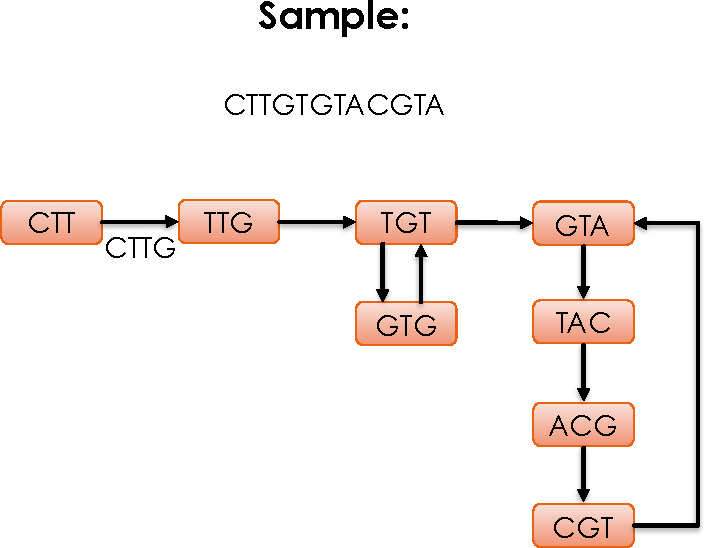
\includegraphics[width=\linewidth]{figs/dbg1-cropped.pdf}
  \caption{de Bruijn graph for a sample with one sequence.}
  \label{fig:dbg-a}
\end{subfigure}%
\begin{subfigure}{.5\textwidth}
  \centering
  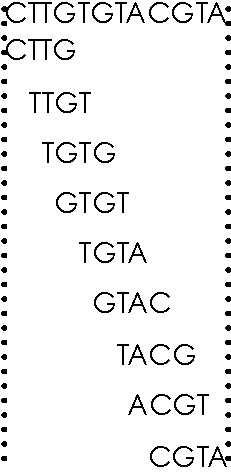
\includegraphics[width=.4\linewidth]{figs/dbg2-cropped.pdf}
  \caption{This example shows how one can reconstruct the reference sequence 
  having a walk through nodes and edges in a de Bruijn graph and taking care of overlaps.}
  \label{fig:dbg-b}
\end{subfigure}
\caption{Building a de Bruijn graph and reconstructing the reference sequence from it}
\label{fig:dbg}
\end{figure}

The \dbg is a useful structure for indexing a reference or set of sequencing reads because it enables fast querying. One drawback is that for the $k-1$ overlaps between consequent edges, the original data structure is very space-inefficient. For example, ABYSS~\cite{simpson2009abyss} represents the \dbg as a hash table with each \kmer as the key and a byte keeping all the connections to other nodes as its value. It needs $1$ bit to show the existence of each of the edges in forward or reverse-complement case (as we have four characters in our alphabet, we can expand the current node to reach to the next one in at most four different ways in forward direction). The space such a data structure takes is $\abs{E_s}(\frac{k}{4}+1)\frac{1}{\gamma}$ bits where $\gamma \leq 1$, is the hash table loading factor. This storage is considerably large for even one genome data set, such as the human genome (starting from 40GB while depending on the loading factor can grow to 100GB or more). Yet, a few different data structures and algorithms have been proposed to reduce the size of a \dbg and represent it efficiently. One category of these data structures use Bloom Filter to represent a \dbg~\cite{pell2012scaling,salikhov2013using,chikhi2012space,chikhi2013space,holley2016bloom}. Other than these, there are a few proposed representations that rely on succinct data structures~\cite{gbmp2014sea} and rank and select operations including the original work by Conway and Bromage~\cite{conway2011succinct} and later the work in~\cite{BoweOn12} that is called the BOSS representation of \dbg from the authors’ initials. BOSS is an efficient edge-centric representation of \dbg that takes around 3 bits per \kmer, which is considerably smaller than the hash table representation. This representation provides a mechanism for navigation through the \dbg and also an interface to interact and get access to the ID of each \kmer. In section \ref{sec:rainbowfish}, I explain in more detail, our work on the color representation for a \dbg built on top of the BOSS structure, using the interface they provide.


\subsection{Compacted de Bruijn Graph}
\label{subsubsec:cdbg}
In addition to all the work that has been done on improving representations for \dbgs, such that a small number of bits are required for each \kmer, there is also a major preparation step in most \dbg preparation pipelines, named compaction. In this step, long paths of \kmers that do not branch are compacted. The process of compacting the \dbg is meant to merge all \kmers in a path in the \dbg with outgoing and incoming degrees less than or equal to one into a single node which is called a \emph{unitig}. The output of this step is called a compacted de Bruijn graph (cdbg), that connects these unitigs and is a variant of the original \dbg with \kmers as nodes. This can be used in the same way as a \dbg for different downstream applications, such as mapping, alignment, variant detection, etc. This method reduces memory by eliminating the great amount of load that overlaps of $k-1$ in consequent \kmers put on memory for cases in the graph that there is only one \textit{possible next} node. For instance, the output node after merging two consequent nodes in a node-centric \dbg with overlap of $k-1$ would be a unitig of length $k+1$ where first base is the first in the source node, the last base is the last in the destination node and the $k-1$ middle bases are shared between source and destination. This compaction step can have a great impact on reducing the memory and is very useful in cases that we are dealing with repeat-heavy sequences~\cite{liu2016debga}. Recently, researchers have designed and implemented algorithms for building a \ccdbg directly from raw data instead of building the memory-inefficient \dbg first and then compacting it in tools such as TwoPaCo~\cite{minkin2016twopaco} and BCalm2~\cite{chikhi2016compacting}. However, indexing a \ccdbg is still a challenge that needs more investigation. 

So far, we know of two other tools, kallisto~\cite{Bray2016Kallisto} and deBGA~\cite{liu2016debga} that are used for indexing \ccdbgs. Although these tools are very efficient in searching for a \kmer, the memory they need is large, so that in case of very large datasets their memory exceeds the limits of a moderate server. In section \ref{sec:pufferfish}, we propose a memory-efficient indexing data structure for a \ccdbg that has an asymptotically constant \kmer lookup time just as these tools. We first use one of the existing tools that we discussed earlier to build the \ccdbg~\cite{minkin2016twopaco}. Later in the same section, we explain our novel data structure to index such \ccdbgs while keeping a balance between space and query time. One great advantage of a specific variant of our indexing structure (sparse indexing) is the flexibility that it provides by giving the option of trading time for space by means of a tunable parameter.

\subsection{Colored de Bruijn Graph}
A \cdbg is a generalized form of a \dbg that allows representing multiple samples in one unified graph while keeping the identity of (and information specific to) each sample~\cite{Iqbal2012Novo}. The samples may be the result of different experiments for the same species, known variants of the same sequence, or different sequencing samples. By counting all of the samples together as one and building a \dbg from them we will lose the variations happening across samples. Colored de Bruijn graphs were originally proposed by Iqbal et. al~\cite{Iqbal2012Novo}  in a tool named \emph{cortex}, useful for variant discovery and genotyping. Each sample is represented with a unique color in a \cdbg and hence all the \kmers coming from that sample will carry that color with them. To be exact, each \kmer or edge in a \cdbg has a color set showing all the samples that this \kmer has appeared in. Maintaining each color separately, we can differentiate between bubbles that are induced by \emph{repeats} when we see the coverage evenly distributed along different paths from \emph{errors} where one side of the branch has a low coverage~\cite{Iqbal2012Novo}. There are other data structures implemented in tools such as BFT~\cite{holley2016bloom} and VARI~\cite{MuggliBoNo17} for representing and processing \cdbgs. However, in most of the cases the color representation is the dominant part in the total space the \cdbg takes compared to the small portion that is taken by the \dbg representation itself. In section~\ref{sec:rainbowfish} we propose a succinct data structure to represent colors in a \cdbg paired with any \dbg representation that provides a unique index for each \kmer. We theoretically prove the succinctness of our data structure and compare our space and query time results with VARI which uses a similar API to construct the index and find bubbles in the \cdbg.


%Gcsa?


\section{Genome And Transcriptome Indexing}
\label{subsec:indexing}
Aligning and mapping sequence reads to a reference genome or transcriptome is an important and unavoidable step of many pipelines in genome and transcriptome analysis. For almost all types of quantification and gene and RNA sequence expression analyses, we first need to align short reads to the reference gene and transcript. However, in most of the analyses, this step is the time-consuming bottleneck. To speed up the alignment process, researchers have used different reference sequence indexing methodologies to first find an exact match to a seed from read and continue aligning from that point. With the increasing accumulation of genomic data, there is a need to index these massive populations of genomes, transcriptomes, and sequencing reads. Existing structures for indexing large strings typically fall into two categories; those that are hash-based and provide very fast access to indexed patterns of fixed-length (\kmers)~\cite{liao2013subread} and the linear self indexing methods that are space-frugal and provide asymptotically efficient but practically slower pattern search for arbitrary length patterns, such as Bowtie2~\cite{langmead2012fast} and BWA-MEM~\cite{li2013aligning} that make use of Borrows Wheelers Transform, or suffix array based indices such as STAR~\cite{dobin2013star}. There have been recent efforts to extend both approaches to the context of indexing different types of sequence graphs~\cite{paten2017genome}, with tradeoffs between space and time efficiency. On the succinct self-index side, one notable example is gramtools, the tool in which the graph itself is represented as a modified BWT \cite{maciuca2016natural}. For the recently developed \kmer lookup based approaches, however, it is more prevalent to use graphs as the underlying data structure. The examples are tools like deBGA~\cite{liu2016debga}, genomeMapper~\cite{schneeberger2009simultaneous}, and BGREAT~\cite{limasset2016read}. 

These efforts are interesting, in part, because the \ccdbg, explained in section \ref{subsubsec:cdbg}, has recently emerged as a desirable sequence indexing data structure, because of the efficiency with which it handles repetitive sequences. By definition, any \kmer present in the reference sequence will occur in exactly one \emph{unitig} of the \ccdbg. The absence of duplicate \kmers in the unitig set allows efficient indexing of these \kmers with a minimum perfect hash function (MPHF)~\cite{limasset2017fast}. In section \ref{sec:pufferfish}, we present pufferfish, an efficient indexing representation of the \ccdbg annotated with information like color, position, orientation, and frequency of each \emph{unitig}. We present two variants of the pufferfish data structure, dense and sparse. The first is optimized for fast queries and the second provides the user with the ability to trade off space for speed in a fine-grained manner.
